\subsection{Phase transitions and critical exponents} 
This set of notes will revolve around explaining the phenomena of phase transitions. In physics so far, we've described systems in terms of smooth and differentiable functions. For example, smooth paths given by solving the Euler-Lagrange equations for $N$ particles. However, in reality, many physical systems exhibit discontinuous behaviour. The most obvious of these would be a phase transition from liquid to gas, say. Or, for example, thje change in magnetisation for a system from an ordered state to a disordered state. One may ask, how can systems comprised of smooth dynamics exhibit discontinuous behaviour? 

\begin{figure}[h]
	\centering
	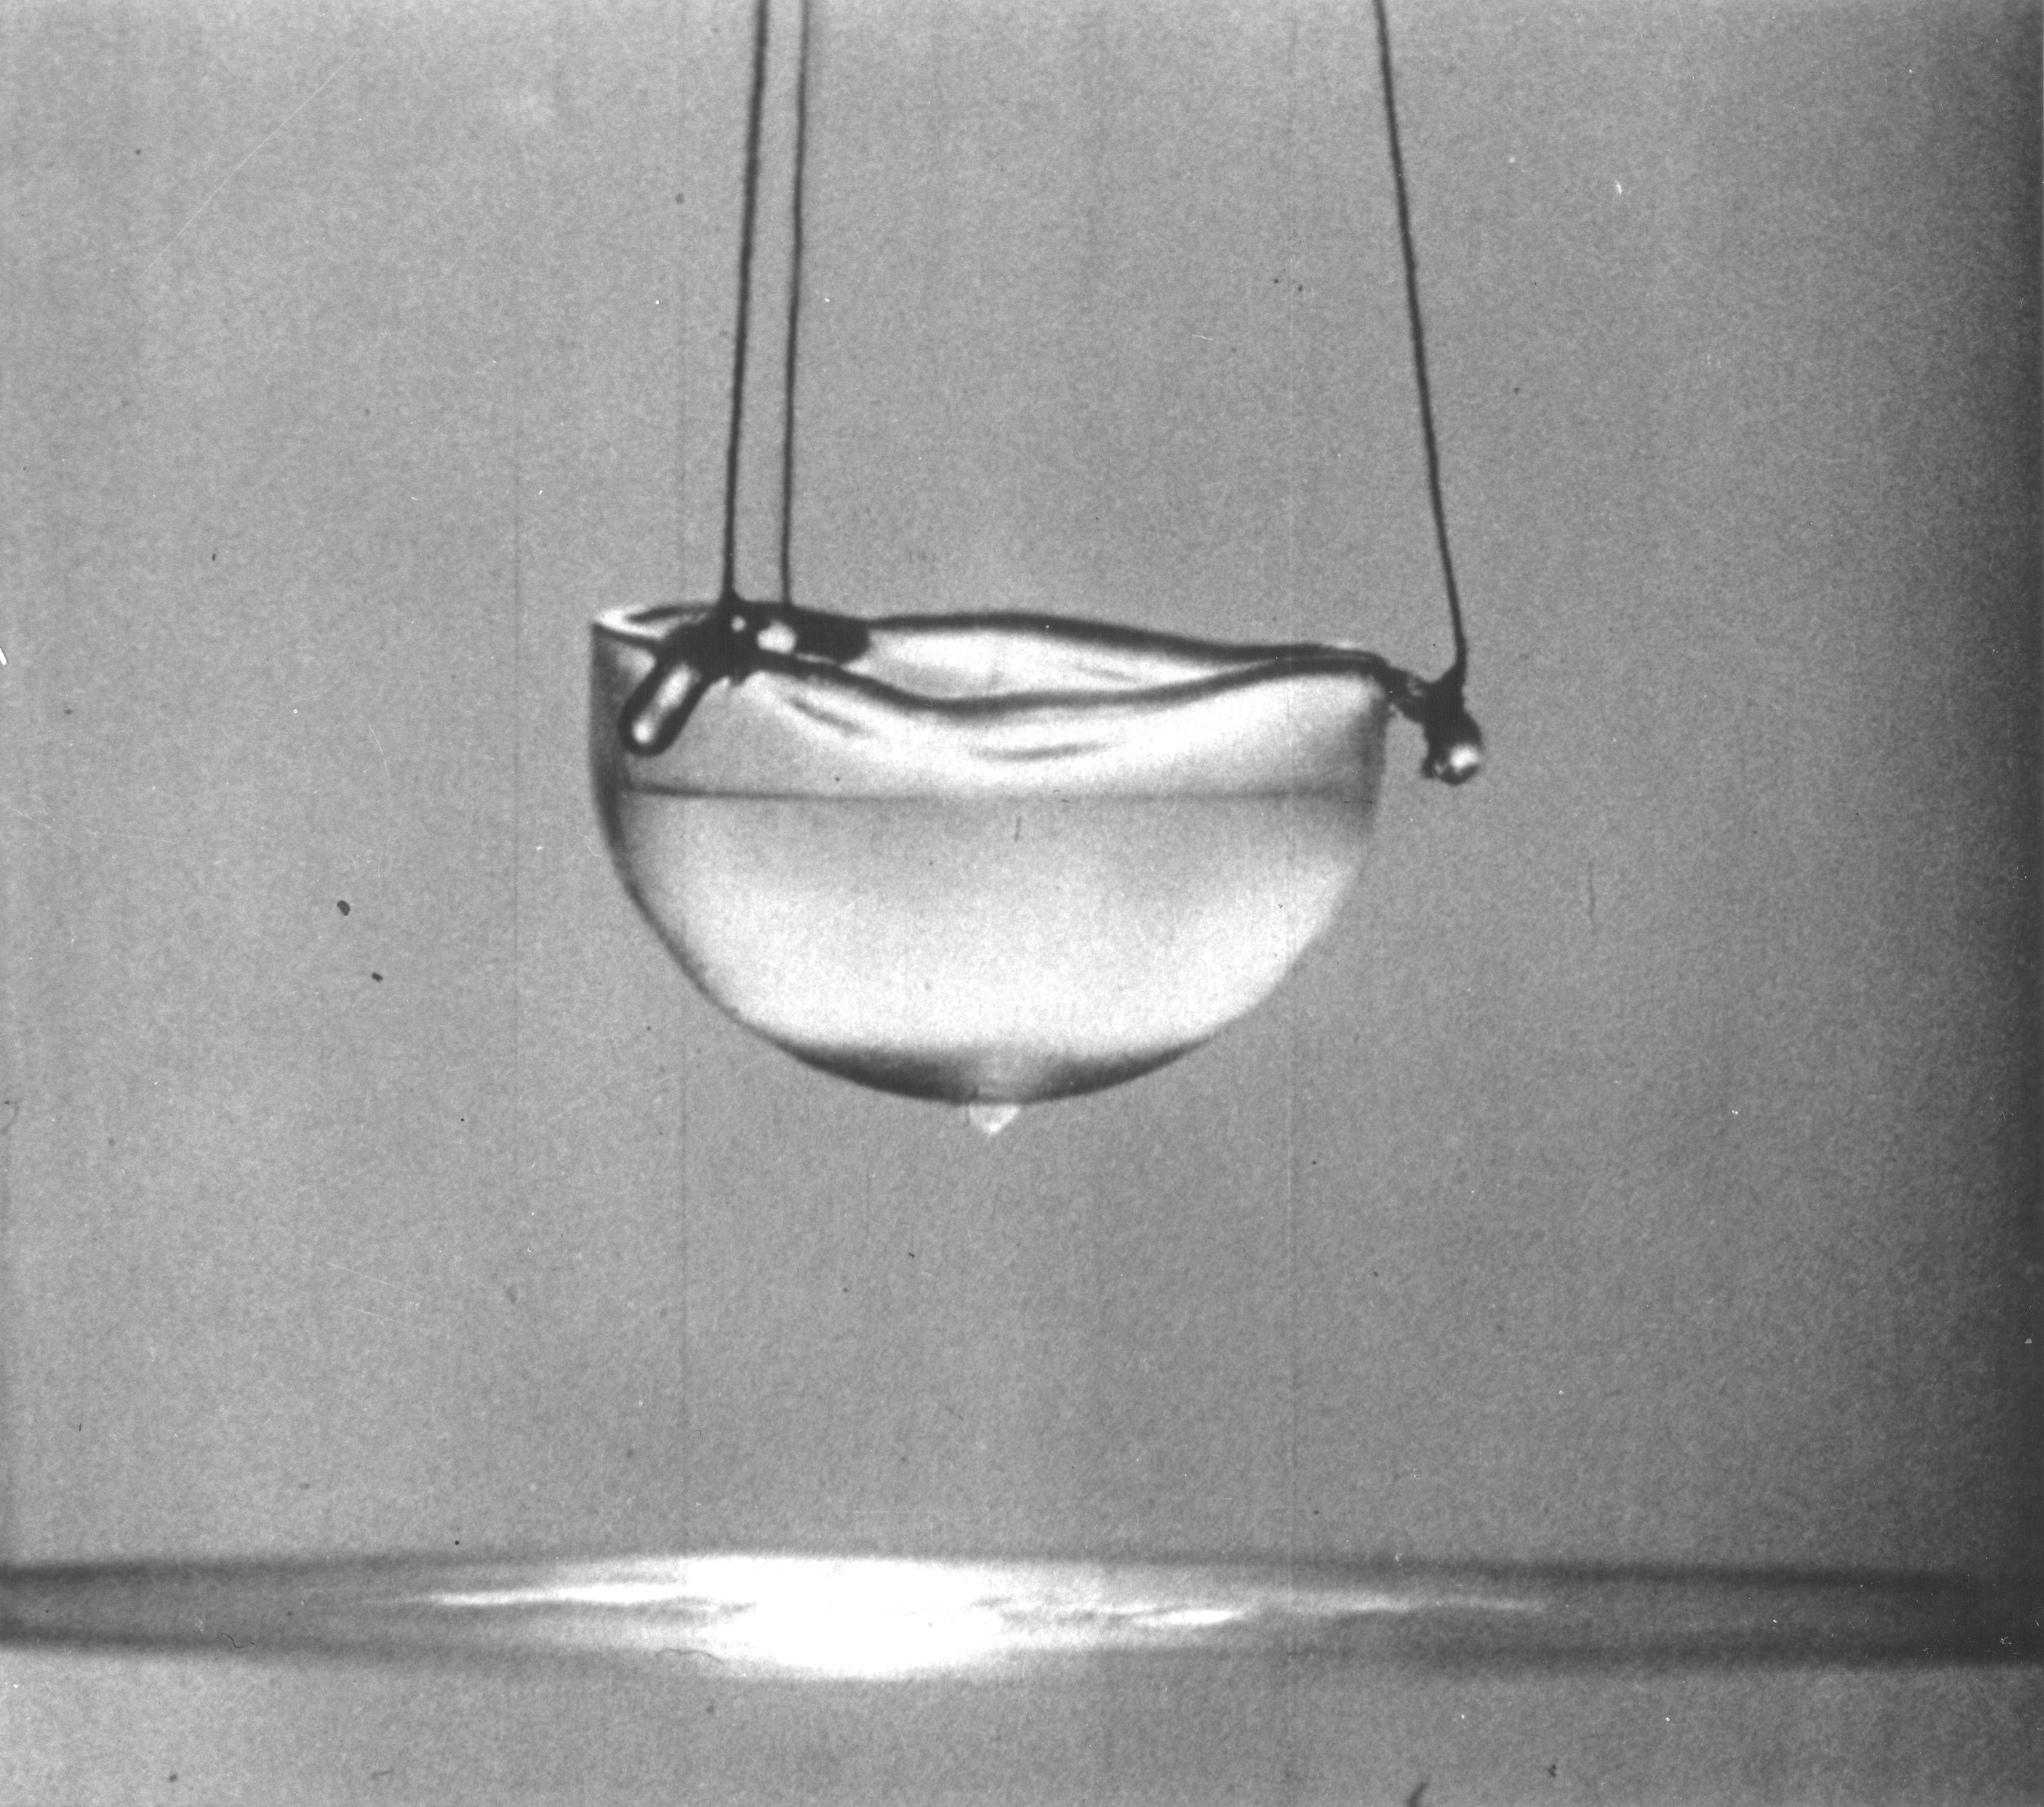
\includegraphics[scale=0.1]{Liquid_helium_Rollin_film.jpg}
	\caption{Helium in a 'superfluid' phase}
\end{figure}

These discontinuities appear as a result of taking an $N \rightarrow \infty$ limit for the number of particles, and our previous functions which are smooth begin to get 'squashed' into a discontinuous shape. We'll study this behaviour throughout these set of notes. The discontinuities of phase transitions occur at special values of descriptors of our physical system (for example temperature, magnetisation, pressure), which we call \textbf{critical points}. How a system behaves near critical points give rise to critical exponents. For example, the mean-field theory prediction of how magnetisation varies as $T$ reaches it's critical temperature is \[ 
m \sim (T - T_c)^\alpha,\quad \alpha = \frac{ 1}{2} \] 
where $\alpha$ is a critical exponent in this case. Or, somewhat conversely, we have another critical exponent derived from how magnetisation changes due to a change the applied magnetic field $B$, which again mean-field theory predicts to have the relationship \[ m \sim B^{ \frac{ 1}{3}} \] and in this case $\frac{ 1}{ 3}$ is another example of a critical exponent appearing in nature. 
Other quantities we might want to examine the behaviour of as we approach critical points in different variables are 
\begin{itemize} 
	\item heat capacity per unit volume, often denoted $c$, changing with as $T \rightarrow T_c $
	\item magnetic susceptibility, which is how the magentisation of a system changes in response to an ambient magentic field: \[ \chi = \frac{ \partial m}{ \partial B } \] and how this quantity also varies as temperature approaches the critical temp $T \rightarrow T_c$
	\item how density of particles, $\nu_{ \text{ gas} / \text{liquid}}$ changes when either pressure or temperature approaches a critical point 
	\item compressibility and more! 
\end{itemize}  
 
